\documentclass[pdftex]{article}
\usepackage[pdftex]{graphics}
\usepackage{subfigure}
\usepackage{hhline}
\usepackage[usenames,dvipsnames]{color}
\usepackage{colortbl}
\usepackage[screen,pdftex]{mcdlecture}
\newcommand{\bs}{\relax}
\newcommand{\es}{\newpage}
\fboxsep=.01\textwidth \fboxrule=1pt
\newsavebox{\savepar}
\newenvironment{boxit}{\begin{lrbox}{\savepar}
    \begin{minipage}[b]{0.975\textwidth}}
    {\end{minipage}\end{lrbox}\framebox{\usebox{\savepar}}}


%%%%%%%%%%%%%%%%%%%%%%%%%%%%%%%%%%%%%%%%%%%%%%%%%%%%%%%%%%
%% THE FOLLOWING ARE THINGS THAT WE MIGHT CHANGE FROM YEAR TO YEAR OR
%% VENUE TO VENUE
    \lhead{MCMC in Statistical Genetics}
    \lfoot{Dr Eric C. Anderson and Dr Matthew Stephens}
%	\lfoot{Dr Eric C. Anderson and Dr John Novembre}
%    \rfoot{UW - Summer Institute, July 2013}
%	 \rfoot{Edinburgh - European Institute, June 2012}
\rfoot{Brazil - Summer Institute, February 2014}

% on this one, be sure to update the venue and the module number
%\newcommand{\coursetitlepage}{European Institute in Statistical Genetics
%\newcommand{\coursetitlepage}{Summer Institute in Statistical Genetics
\newcommand{\coursetitlepage}{Brazilian Edition of the Summer \\Institute in Statistical Genetics

Module 9:

MCMC for Genetics}

%% Then update the schedule.  Note that I have broken that
%% out into a separate file like: schedule_table_edinburgh2012.tex
%% which is input in Overview.tex

%% Then be sure to change any time-sensitive events in the 
%% probability discussion in Matthew's first lecture.

%% And also update "structure_fun" link to my wiki to the right
%% year and venue.
%%%%%%%%%%%%%%%%%%%%%%%%%%%%%%%%%%%%%%%%%%%%%%%%%%%%%%%%%%


\begin{document}

\DeclareGraphicsExtensions{.jpg,.pdf,.png}%



%% Eric added a few things:
% some commands that Eric made for making a title while starting
% a new lecture and for making titles of new slides.
\newcommand{\newlecture}[1]{\newpage\begin{center}\section*{#1}\end{center}}
\newcommand{\newslide}[1]{\newpage\subsection*{#1: \hfil}}
 \newcommand{\Exp}{\Bbb{E}}
 \newcommand{\Var}{{\mathrm{Var}}}
 %% Some pretty etc.'s, etc...
\newcommand{\cf}{{\em cf.}}
\newcommand{\eg}{{\em e.g.},}
\newcommand{\ie}{{\em i.e.},}
\newcommand{\etal}{{\em et al.}\ }
\newcommand{\etc}{{\em etc.}}

%% some handy things for making bold math
\def\bm#1{\mathpalette\bmstyle{#1}}
\def\bmstyle#1#2{\mbox{\boldmath$#1#2$}}
\newcommand{\thh}{^\mathrm{th}}
\newcommand{\bpi}{{\pi}}
\newcommand{\mP}{\mathbf{P}}

\rhead{Session 10 - \thepage}

\newcommand{\bY}{{\bm{Y}}}
\newcommand{\bX}{{\bm{X}}}
 
 
\newlecture{The Bottom Drawer---A Variety of Topics}
The goals of this lecture are:
\begin{itemize}
\item Introduce {\em importance sampling}---a Monte Carlo variance reduction technique
\item Explain how MCMC can be used to compute likelihood ratios
\item Demonstrate MCMC in simple pedigrees and discuss problems of reducibility
\item Discuss poor mixing more generally and describe \\ Metropolis-coupled MCMC
\end{itemize}


\newslide{The opposite of importance sampling---``minimal relevance" sampling}
\vspace*{-.45in}
Let's say you wanted to estimate the area under the curve $g(x)$ below by Monte Carlo:
\begin{center}
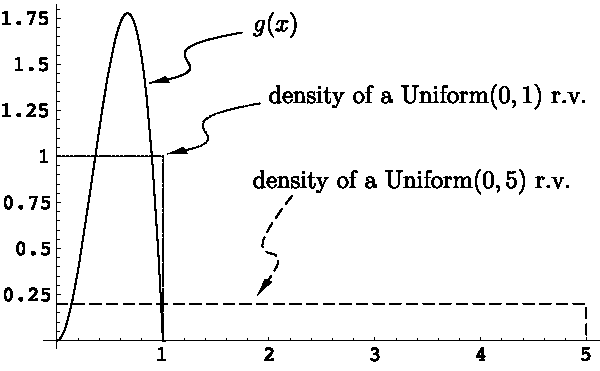
\includegraphics[width=.7\textwidth]{illus/betacurve.pdf}
\end{center}
\enlargethispage*{100pt}
Note that we are back to ``vanilla" Monte Carlo (not MCMC) for the next five slides or so\ldots



\newpage
$\bullet$ We could simulate random variables $U\sim\mathrm{Uniform}(0,1)$
\[
\int_0^1g(x)dx = \int_0^1g(x) 1 dx = \Exp[g(U)] \approx \frac{1}{n}\sum_{i=1}^n g(u^{(i)})
\]
And that would work pretty well.

$\bullet$ We could also simulate random variables $W\sim\mathrm{Uniform}(0,5)$
\[
\int_0^1g(x)dx = 5\int_0^1g(x) \frac{1}{5} dx = 5\Exp[g(W)] \approx \frac{5}{n}\sum_{i=1}^n g(w^{(i)})
\]

$\bullet$ Each method is correct, but the second is clearly inefficient.  Any values of $w^{(i)}$ greater than 1 don't provide us with any information about the area under $g(x)$!!  

$\bullet$ The second method has larger Monte Carlo variance.

\newslide{Importance sampling}
\begin{itemize}
\item Importance sampling is choosing a good
distribution from which to simulate one's random variables for Monte Carlo.
\item It involves
multiplying the integrand by 1 (usually dressed up in a ``tricky
fashion") to yield an expectation of a quantity that varies less than the
original integrand over the region of integration.

\item For example, say we wish to approximate $\int_{x\in\mathcal A}g(x)dx$ and we can ``dream up" a distribution $h(x)$.
\[
\int_{x\in\mathcal A}g(x)dx = \int_{x\in\mathcal A}g(x)\frac{h(x)}{h(x)}dx 
= \int_{x\in\mathcal A}\frac{g(x)}{h(x)}h(x)dx
\]
which is
\[
\Exp_h\left[\frac{g(X)}{h(X)}\right]
\]
where $\Exp_h$ denotes the expectation with respect to the density $h$, so long as $h(x)>0$ for all values $x$ for which $g(x)\neq 0$.
\newpage
So we could approximate $\int_{x\in\mathcal A}g(x)dx$ by:
\[
G_n^h = \frac{1}{n} \sum_{i=1}^n  \frac{g(x^{(i)})}{h(x^{(i)})}
\]
where each $x^{(i)}$ is simulated from the density $h$. 

\item Using the Cauchy-Schwarz inequality, it is not too difficult to show that the Monte Carlo variance of $G_n^h$ is minimized when $h(x)\propto |g(x)|$.

\item Even more straightforward, if we consider only the case where $g(x)>0$, it is immediately apparent that the Monte Carlo variance is minimized (is zero, in fact) when $h(x)\propto g(x)$.  

\item Of course, if you could simulate independent r.v.'s from a distribution exactly proportional to $g(x)$, that implies you know the value of the integral anyway. So this is a little circular---but it does emphasize that importance sampling works best when $h(x)$ is close to proportional to $g(x)$. 
\end{itemize}

\newslide{Choosing a good importance sampling distribution}
A good importance sampling function $h(x)$ should have the following
properties:
\begin{enumerate}
\item $h(x) > 0$ whenever $g(x) \neq 0$
\item $h(x)$ should be close to being proportional to $|g(x)|$
\item it should be easy to simulate values from $h(x)$
\item it should be easy to compute the density $h(x)$ for any value $x$ that you
might realize.
\end{enumerate}
Fulfilling this wish-list in high dimensional space (where Monte Carlo techniques
are most useful) is quite often a tall task.

\newslide{Simple example: Estimating the area under a $\mathrm{Normal}(0,1)$ curve with $n=1,000$}
\begin{center}
%\begin{minipage}{.3\textwidth}
%	\begin{center}
		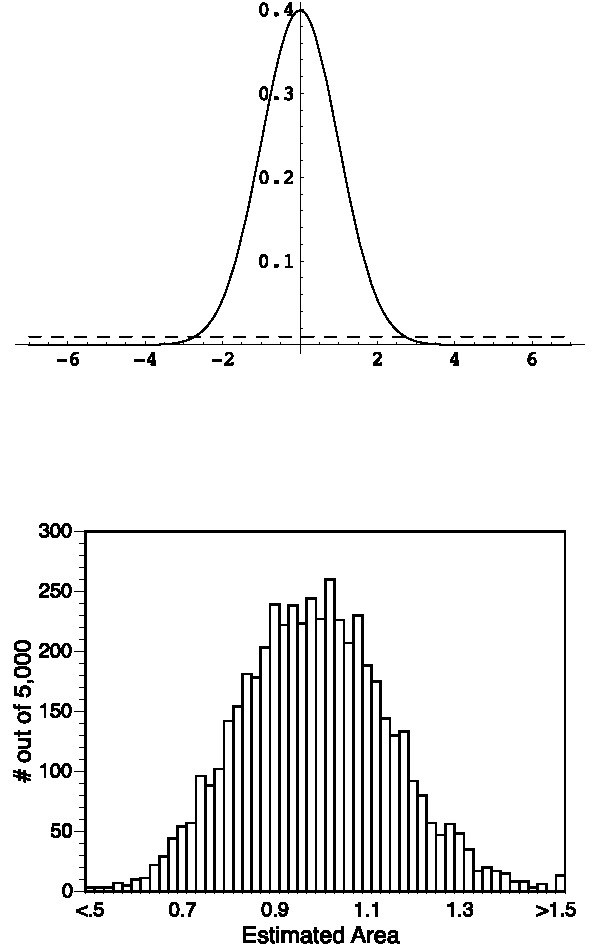
\includegraphics[width=.3\textwidth]{illus/uniformboth.pdf} \hfill
%	\end{center}
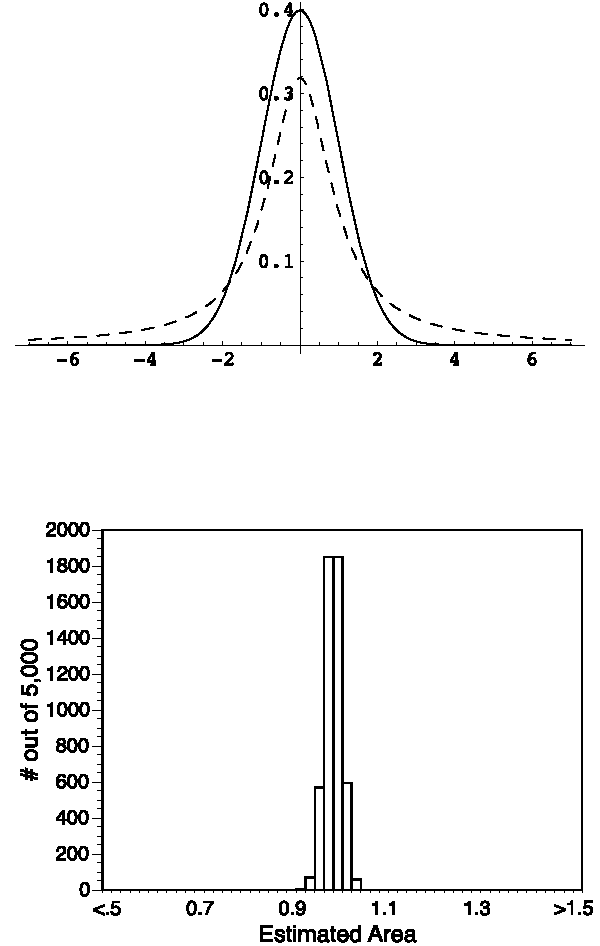
\includegraphics[width=.3\textwidth]{illus/t1both.pdf}\hfill
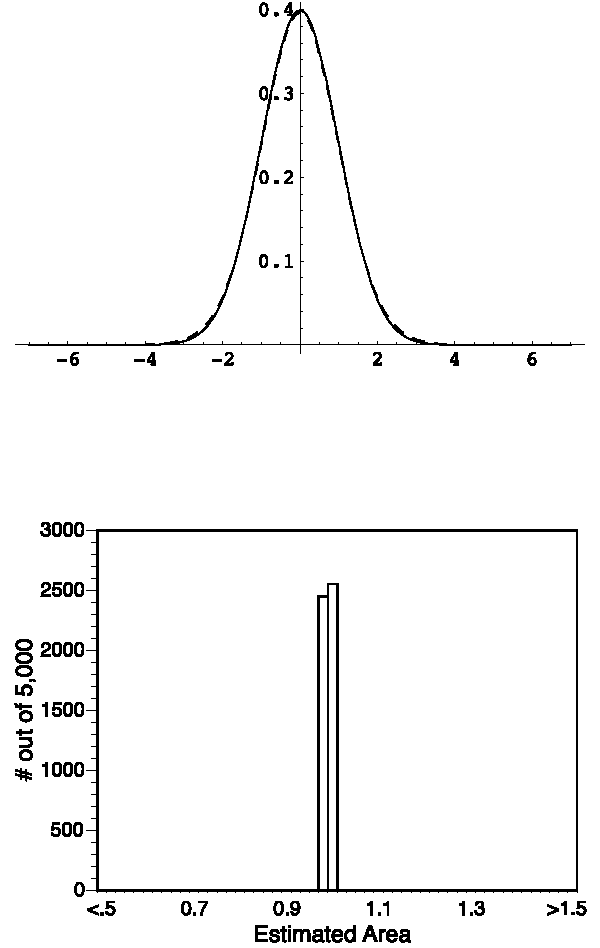
\includegraphics[width=.3\textwidth]{illus/t30both.pdf}
\end{center}
~~$h(x)\equiv\mathrm{Uniform}$\hfill $h(x)\equiv t_1$ Dist. \hfill $h(x)\equiv t_{30}$ Dist.~~~~

\newslide{Example of importance sampling in genetics}
\begin{itemize}
\item Griffiths and Tavare (1994) developed a ``recursion" method for simulating genealogies under the coalescent model conditional on genetic data at the tips of the branches (but not {\em exactly} from their distribution given the data).

\item This method simulates independent genealogies that can be used in Monte Carlo. 

\item It wasn't until somewhat later that Joe Felsenstein and his colleagues were able to dissect the method and show that it is an example of importance sampling. 

\item Viewing the method as an importance sampling task, Matt Stephens and Peter Donnelly (2000) were able to improve upon the method considerably.
\end{itemize}


\newslide{A common pitfall of importance sampling}
\begin{itemize}
\item Whatever is going on in the ``tails" of the distribution is, unfortunately, very important\ldots
\item If $h(x)$ is thinner-tailed than $g(x)$ there could be problems: if for a rarely-realized value $x^{(i)}$, $h(x^{(i)})$ is very small, but $g(x^{(i)})$ is not terribly small, then $g(x^{(i)})/h(x^{(i)})$ could be much larger than typical ratios of $g(x)/h(x)$, leading to an unstable estimator.

\item Consequently, assessing the convergence of importance sampling estimators can, at times, be quite difficult.

\end{itemize}

\newslide{An example of a problematic thin-tailed importance sampling distribution}
Approximate the area under a thick-tailed Cauchy ($t_1$) distribution using a thin-tailed $\mathrm{Normal}(0,1)$ density as the importance sampling distribution, and $n=1,000$:

\begin{minipage}{.4\textwidth}
The distribution of Monte Carlo estimates appears to the right.  The correct area is 1.0.  Notice the number of estimates that are greater than 1.5.
\end{minipage}
\hfill
\begin{minipage}{.5\textwidth}
\begin{center}
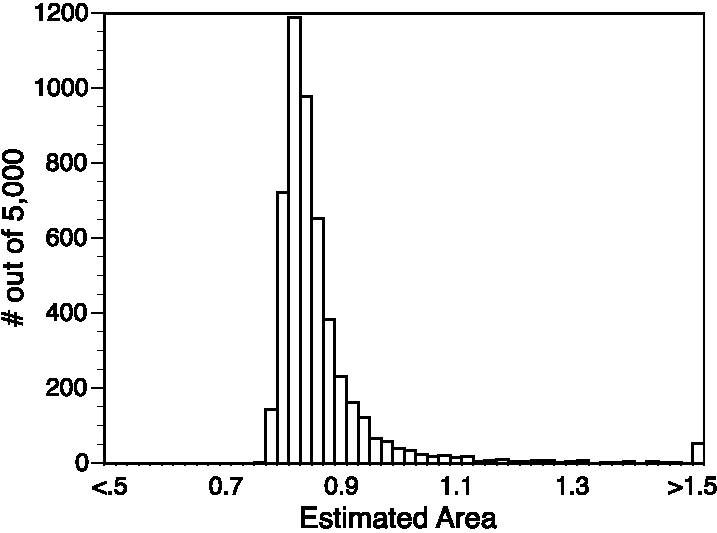
\includegraphics[width=\textwidth]{illus/t1bynorm.pdf}
\end{center} 
\end{minipage}



\newslide{MCMC in a frequentist framework---not just for Bayesians anymore}
Geyer and Thompson (1992) use an importance sampling method to compute likelihood ratios using MCMC.  
\begin{itemize}
\item The basic inference problem is to compute the relative likelihood for different values of $\theta$ given data $\bY$, but the likelihood $P_\theta(\bY)$ is an intractable sum over latent variables $\bX$:
\[
	P_\theta(\bY) = \sum_{\bX} P_\theta(\bY,\bX)
\]
\item We wish to be able to compute $P_\theta(\bY) / P_{\theta_{0}}(\bY)$---the ratio between the likelihood for some arbitrary $\theta$ and the likelihood for a fixed $\theta_0$.
\item Geyer and Thompson found a tricky way of multiplying the above equation by 1 to get a useful result:
\newpage
\addtolength{\jot}{2ex}
\begin{eqnarray*}
P_\theta(\bY) & = &\sum_{\bX} P_\theta(\bY,\bX)\frac{P_{\theta_0}(\bY,\bX)}{P_{\theta_0}(\bY,\bX)} \\
& = &\sum_{\bX} P_\theta(\bY,\bX)\frac{P_{\theta_0}(\bX|\bY)P_{\theta_0}(\bY)}{P_{\theta_0}(\bY,\bX)} \\
\end{eqnarray*}   
So,
\[
	\frac{P_\theta(\bY)}{P_{\theta_0}(\bY)} = \sum_{\bX} \frac{P_\theta(\bY,\bX)}{P_{\theta_0}(\bY,\bX)}
	P_{\theta_0}(\bX|\bY) = 
	\Exp_{\theta_0}\left[\left. \frac{P_\theta(\bY,\bX)}{P_{\theta_0}(\bY,\bX)}  \right| Y \right]
\]
\[
	\frac{P_\theta(\bY)}{P_{\theta_0}(\bY)} \approx \frac{1}{n}\sum_{i=1}^n
	 \frac{P_\theta(\bY,\bX^{(i)})}{P_{\theta_0}(\bY,\bX^{(i)})}~~~~\mathrm{with}~~~
	 \bX^{(i)} \sim P_{\theta_0}(\bX|\bY)
\]
and $P_{\theta_0}(\bX|\bY)$ is a distribution known only up to scale, so it may be simulated from via MCMC.
\end{itemize}


\newslide{Switching gears---a simple example of MCMC on a pedigree with ``data at the bottom"}
\begin{center}
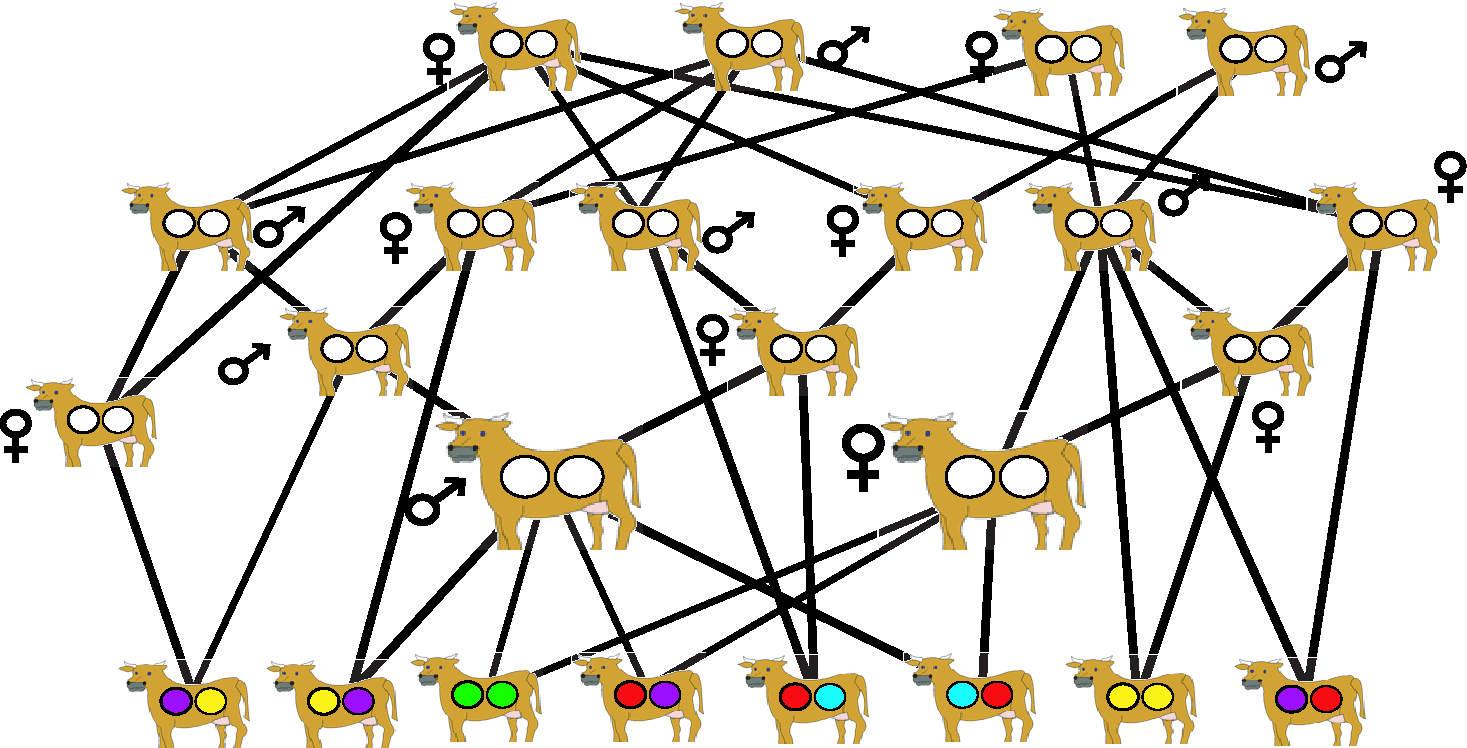
\includegraphics[width=.95\textwidth]{illus/cows_dat.pdf}
\end{center}
The colored balls represent observed allelic types at a locus.

\newslide{Asking questions about the ancestors}
Simple questions:
\begin{itemize}
\item What is the probability that only $n$ copies of the red allele occurred in the founders?
\item What is the probability that ancestor $Z$ carried exactly one copy of the purple allele?
\end{itemize}
More complex questions:
\begin{itemize}
\item What is the probability of the observed data at two loci, given that the recombination fraction between those loci is $\theta$?
\end{itemize}
All such questions can be written as a sum over the unobserved (latent) genotypes of the ancestors, and hence they can be expressed as expectations and approximated by Monte Carlo.  

\newslide{Simulating ancestral genotypes naively will fail}
You can't just ``flip-a-coin" your way up the pedigree the way that Wright and McPhee (1925) could to estimate inbreeding:
\begin{center}
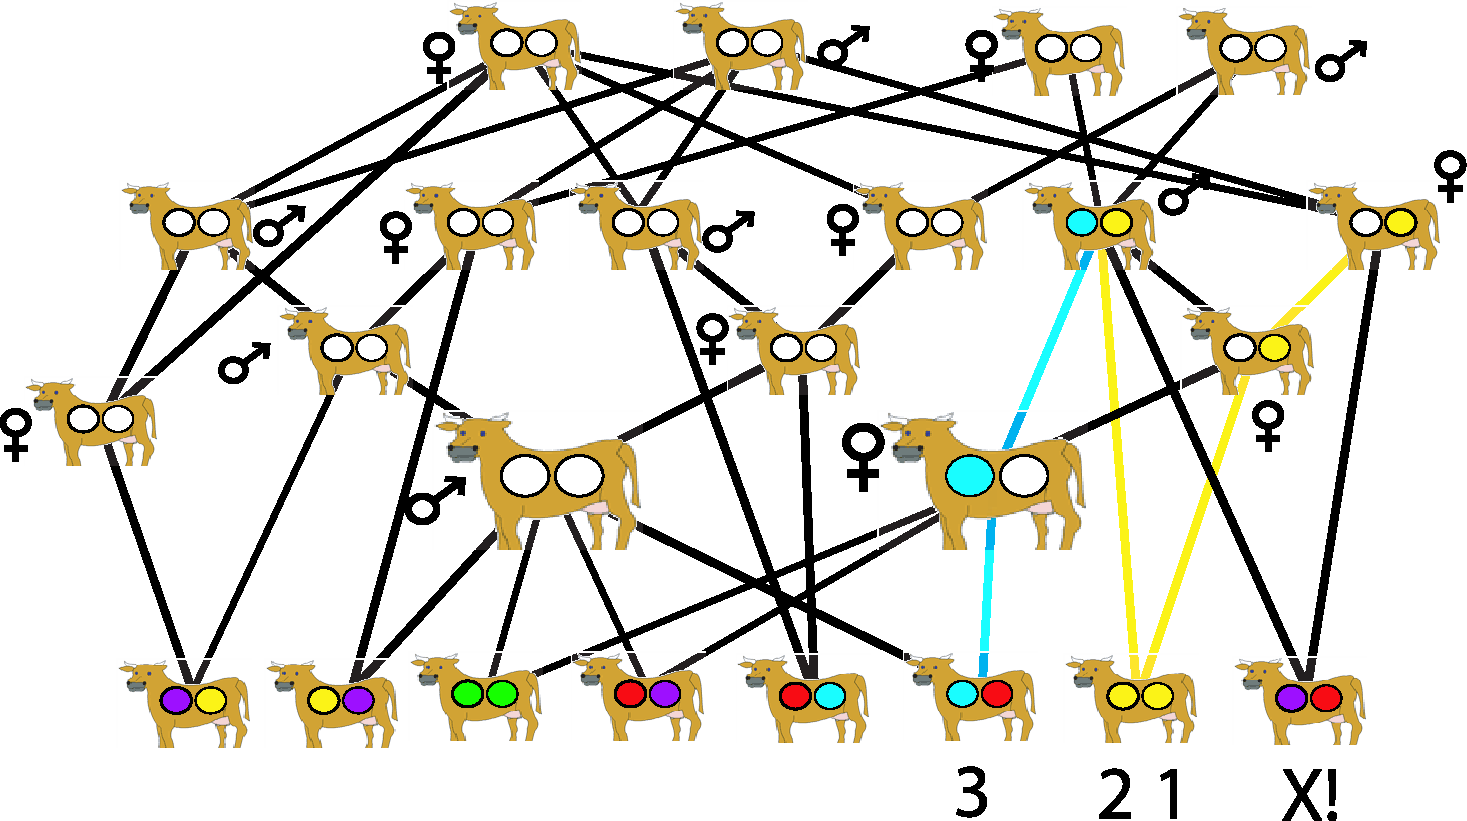
\includegraphics[width=.90\textwidth]{illus/cows_naive.pdf}
\end{center}

\newslide{Another graph-like notation---pedigrees}
\begin{center}
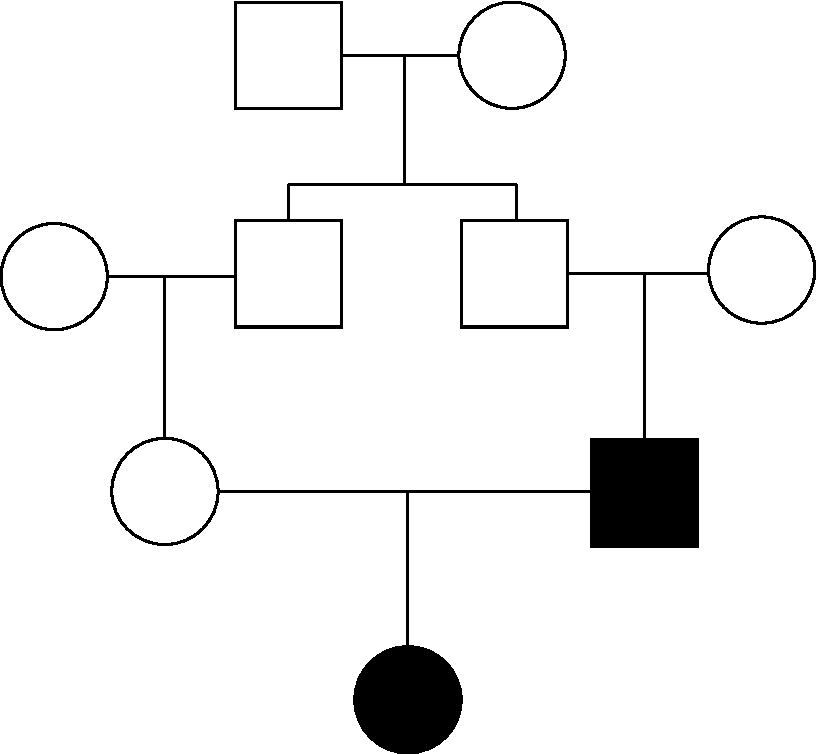
\includegraphics[width=.35\textwidth]{illus/ped1.pdf}
\end{center}
Males are squares.  Females are circles.  Black nodes mean they have observed data (\ie they are part of $\bY$).

\newslide{The full conditional distribution for an individual's genotype at a locus\ldots}
\begin{center}
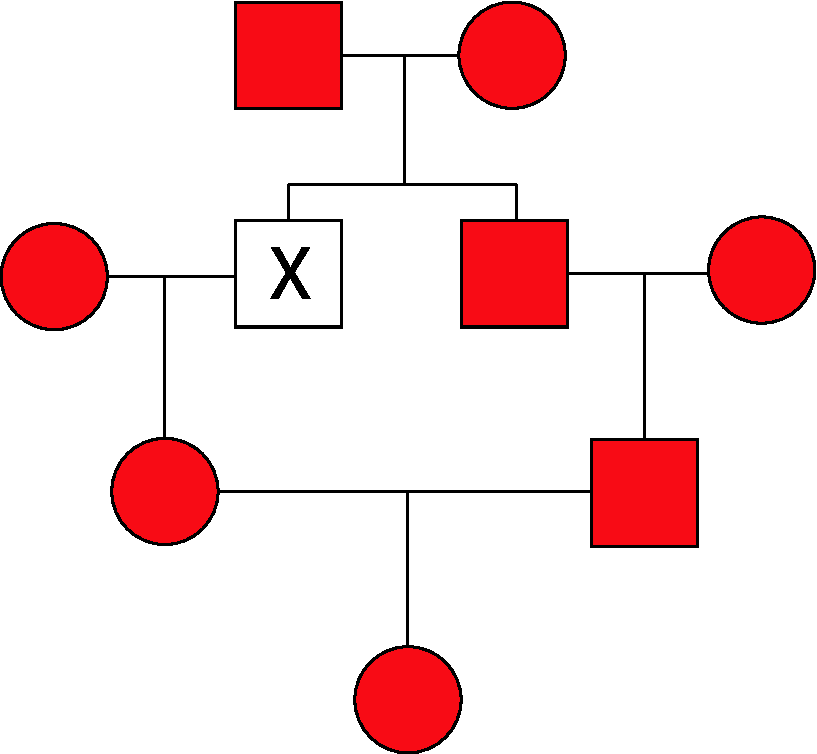
\includegraphics[width=.35\textwidth]{illus/ped2.pdf}
\end{center}
(Red nodes represent the elements that are conditioned on to determine the full conditional for the node labeled ``X".)

\ldots depends only on its neighbors\ldots


\newslide{These are the people in your neighborhood}
\begin{center}
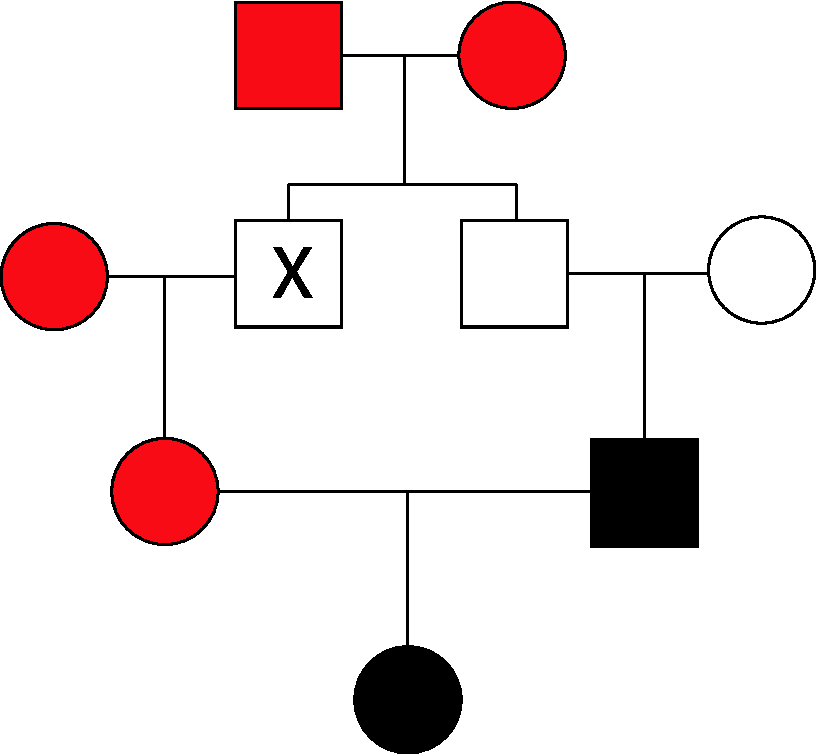
\includegraphics[width=.35\textwidth]{illus/ped3.pdf}
\end{center}
Parents, children, and spouses, (the red ones) are neighbors of node ``X".

So assuming you can find a valid starting configuration, you can buzz around and do Gibbs updates to each individual's genotypes, and thus simulate the latent ancestor genotypes ($\bX$) conditional on the observed data $\bY$.  


\newslide{Irreducibility of single-site Gibbs sampler with two alleles}
Demonstrating this principle on an even simpler pedigree,

If the data look like:
\begin{center}
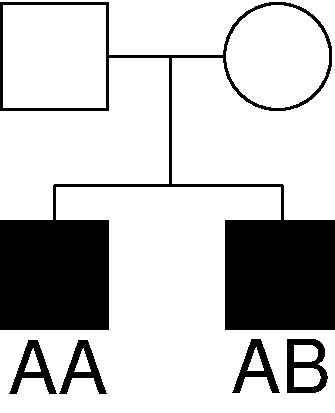
\includegraphics[width=.35\textwidth]{illus/simple_ped1.pdf}
\end{center}

\newpage
Then there are only three possible configurations of genotypes in the unshaded individuals, and these states are reachable from one another in a finite number of steps of single-site Gibbs updating.  Hence this sampler is irreducible here.
\begin{center}
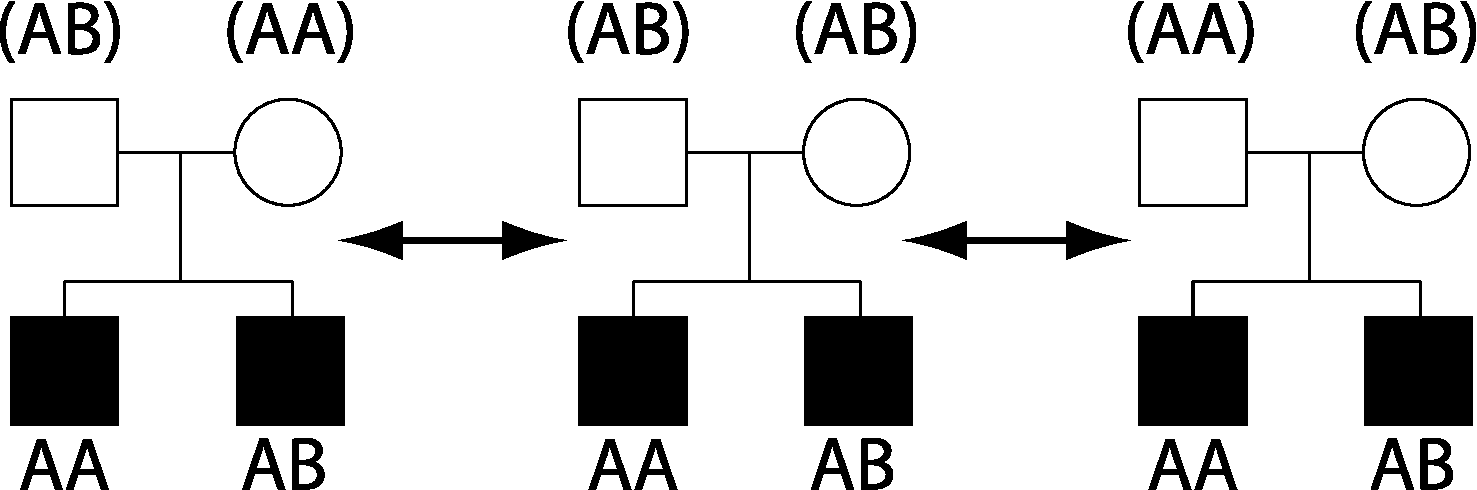
\includegraphics[width=.9\textwidth]{illus/simple_peds_comm.pdf}
\end{center}



\newslide{With multiple alleles, however, the single-site Gibbs sampler is reducible}
For example, with data like\ldots
\begin{center}
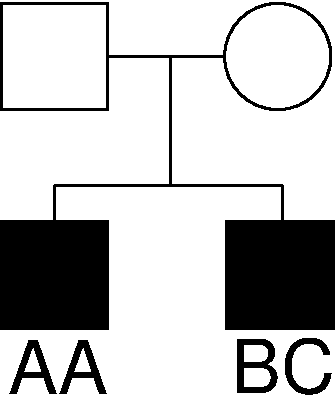
\includegraphics[width=.20\textwidth]{illus/simple_ped2.pdf}
\end{center}
\newpage
\ldots
There are only two possible states for the genotypes of the unshaded individuals and they do not communicate:
\begin{center}
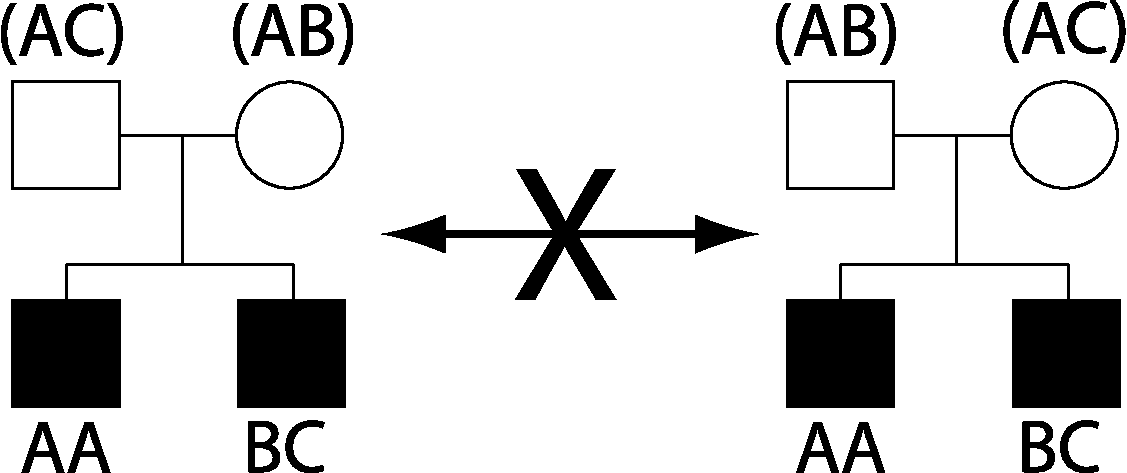
\includegraphics[width=.9\textwidth]{illus/simple_ped2_nocomm.pdf}
\end{center}
So, the single-site Gibbs sampler is not irreducible for most pedigree problems of consequence.  It leads to a reducible Markov chain.

\newslide{Irreducibility ain't the only thing}
While irreducibility is essential for MCMC, it is often possible to have an irreducible sampler, but have {\em poor mixing}.

\ie{} you may be able to show theoretically that your sampler is irreducible, but {\em practically} it may not reach all areas of high probability.

Poor mixing means that the chain does not adequately sample all regions of the space.  

Consider the following one-dimensional example---a mixture of  three normal densities:

\newpage
\begin{center}
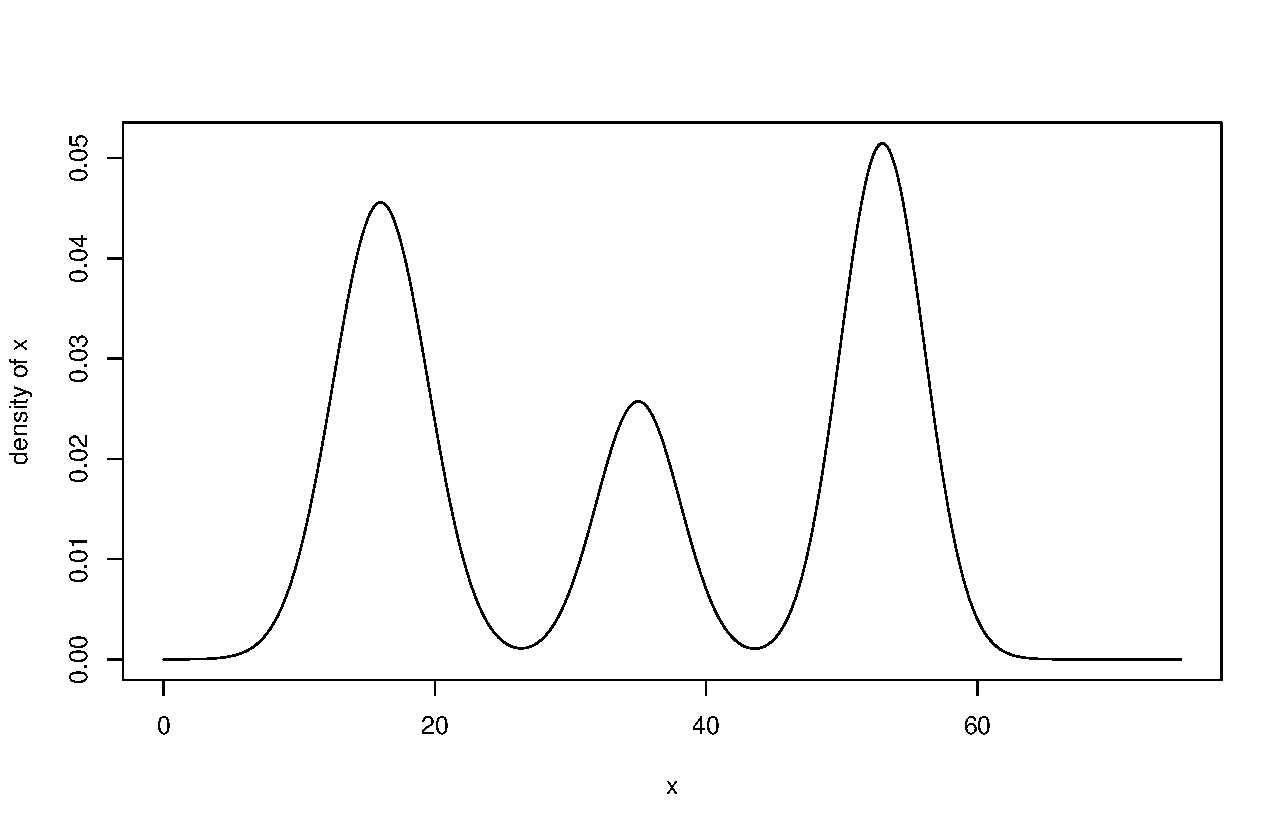
\includegraphics[width=\textwidth]{illus/3peak.pdf}
\end{center}
\enlargethispage*{1000pt}
\fbox{Computer Demo}

\newslide{Designing samplers to mix well}
This is often the hardest challenge in MCMC, especially in high dimensional  space with bumpy or multimodal likelihood surfaces.  

Obvious improvements could come from:
\begin{itemize}
\item Tweaking the proposal distribution (but note that if the variance of the proposal distibution is very high, the acceptance rate may $\downarrow$)
\item Updating several variables jointly. In Gibbs sampling, in particular, this can be useful.  (However, the computations necessary may require considerable extra time).
\end{itemize}

One general method for improving mixing is now called {\em Metropolis-coupled} MCMC (Geyer 1991).  

This is used extensively in the Bayesian phylogenetic analysis package \textsc{Mr~Bayes}.

\newslide{Metropolis-coupled MCMC}
MCMCMC takes advantage of the fact that by raising a probability density to a power $\beta$ between zero and one, the relative heights of peaks, and the relative depths of valleys, may be made less extreme:

\enlargethispage*{100pt}
\vspace*{-.09in}
\begin{center}
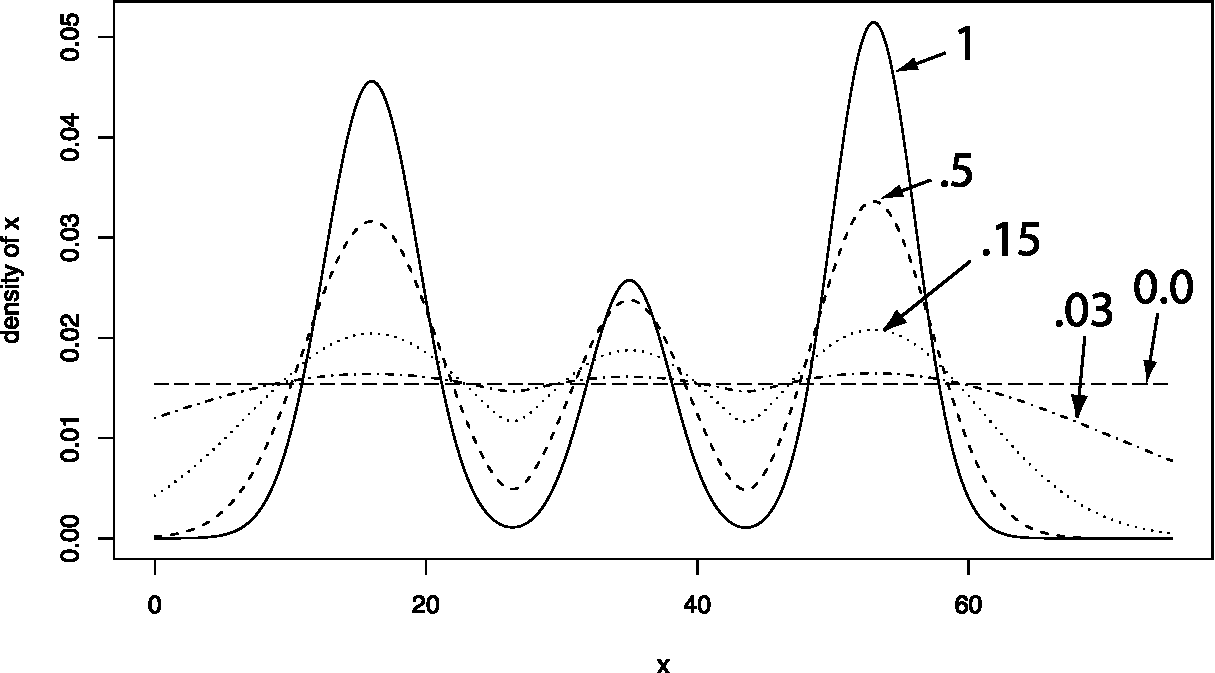
\includegraphics[width=.95\textwidth]{illus/3peak_squashed.pdf}
\end{center}

\newslide{Recipe for Metropolis-coupled MCMC}
\begin{itemize}
\item Let $X$ denote all the different variables being sampled in the MCMC
\item Run one chain, labelled 1, as you normally would with limiting distribution $f(X)$ being the distribution you wish to sample from.  Note: $\beta_1 = 1$.
\item Run $n-1$ other chains (chains $2,\ldots,n$) in the same way, except run them so that the limiting distributions  are ``flattened out" versions of $f$. \ie{} the $i\thh$ chain ($i=2,\ldots,n$) uses a Hastings ratio that looks like:
\[
	\frac{q(X|X')}{q(X'|X)} \frac{[f(X')]^{\beta_i}}{[f(X)]^{\beta_i}}
\] 
where each $\beta_i$ is between 0 and 1.  These chains are often called the ``hot" chains, because they move around more easily---much like a heated molecule.
\item In addition to the normal MCMC updates, also perform ``chain-swapping" updates:
\begin{enumerate}
\item Choose a pair of chains $i$ and $j$ ($1\leq i < j \leq n$) at random and propose swapping their current states ($X_{[i]}$ and $X_{[j]}$, respectively).
\item Accept or reject the proposed swap using the Hastings ratio:
\[
	\alpha = \min\left\{
		1, \frac{[f(X_{[i]})]^{\beta_j}}{[f(X_{[i]})]^{\beta_i}}
		\frac{[f(X_{[j]})]^{\beta_i}}{[f(X_{[j]})]^{\beta_j}}
	\right\}
\]
\end{enumerate}
\item The Monte Carlo sample itself is {\em only drawn from chain}~1!
\item Derivation of the Hastings ratio is easy: given $i$ and $j$ and the current states $X_{[i]}$ and $X_{[j]}$, the proposal distribution is symmetrical, so those terms cancel out.  The bits that remain are just the ratio of limiting distributions of the proposed {\em vs}. the original states.
\item Computationally, you don't have to swap the states (which could mean copying a lot of memory around).  Instead you just swap $\beta$'s.
\end{itemize}
\fbox{Computer Demo}








\newslide{Simulated Annealing}
\vspace*{-1.4em}
\enlargethispage*{100pt}
$\bullet$ Simulated annealing is an optimization technique that relies on ``tricks'' like those employed in Metropolis-coupled MCMC   \\
$\bullet$ Consider what happens if $\beta>1$. {\small (Thick red line is $\beta=1$.  Dotted black line is $\beta=6$. Thin solid blue line is
$\beta=16$.)}
\vspace*{-.19in}
\begin{center}
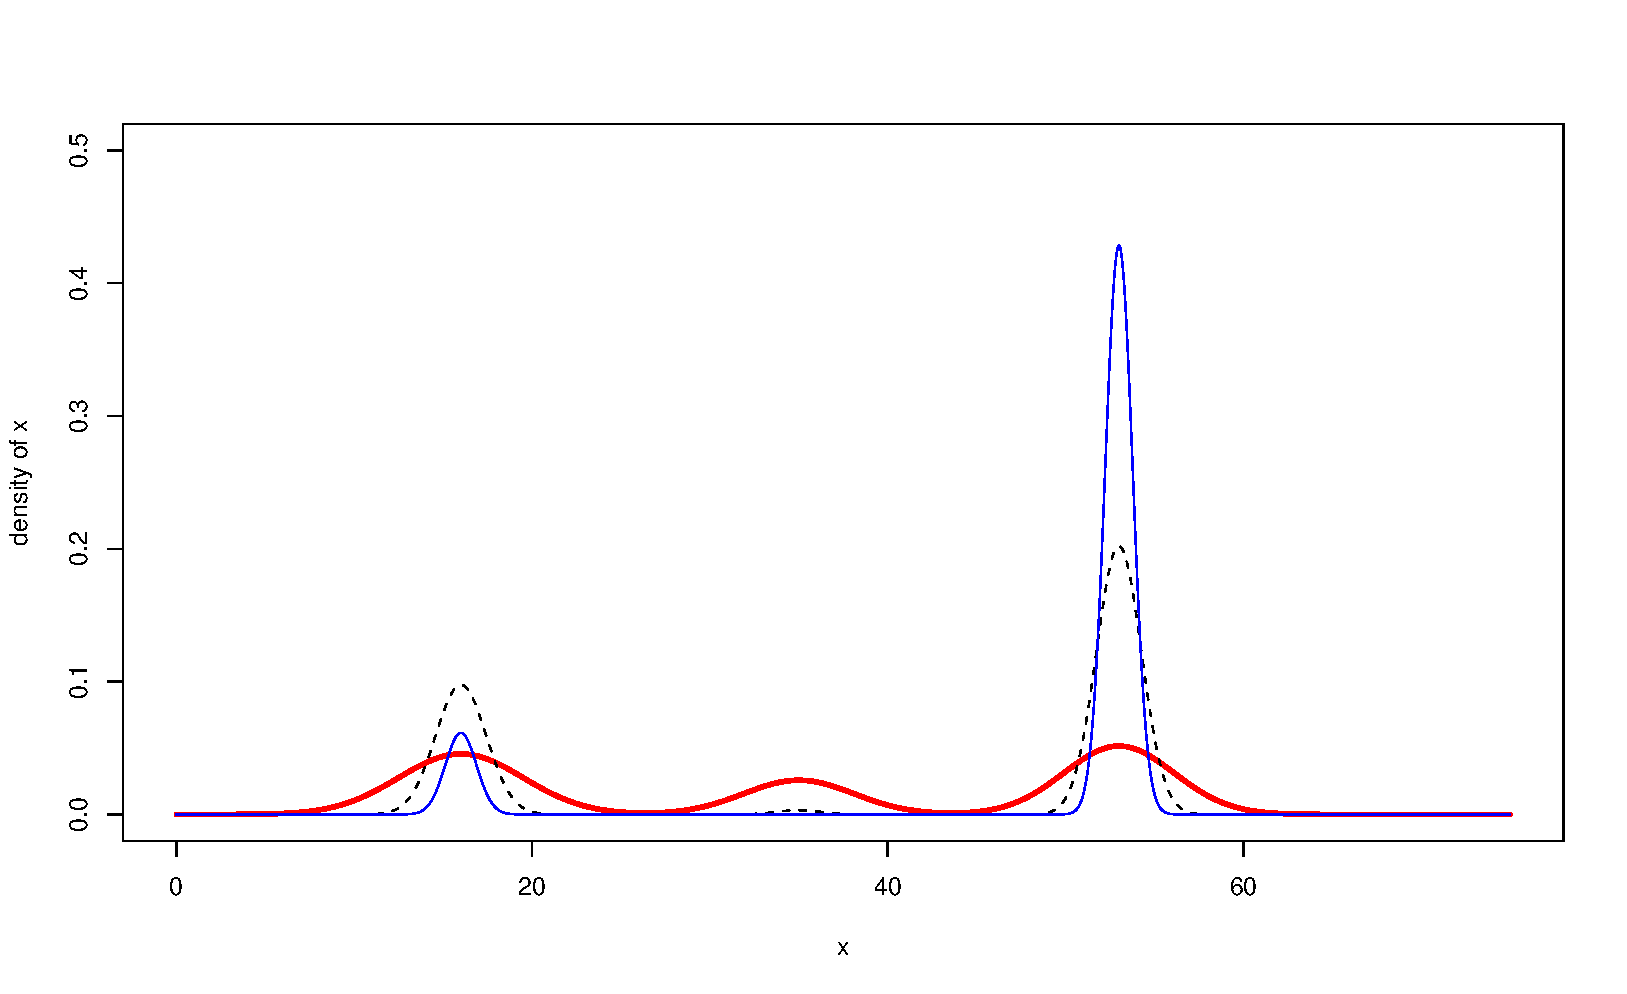
\includegraphics[width=.92\textwidth]{illus/3peaks_annealing.pdf}
\end{center}




\newslide{Recipe for  simple simulated annealing}
 Imagine $f(x)$ is an objective function you wish to maximize.  That is, you want to find the value of $x$ that maximizes $f(x)$. To do so by simulated annealing you\ldots
\begin{itemize}
\item Imagine that $f(x)$ is an unnormalized probability density or mass function
\item Design an M-H sampler to sample $x$'s from target distribution $f(x)$
\item Run a single chain using this M-H sampler while raising $f(x)$ in the M-H ratio to the power of $\beta$:
\[
	\frac{q(X|X')}{q(X'|X)} \frac{[f(X')]^{\beta}}{[f(X)]^{\beta}}
\] 
\item Start with $\beta$ small (less than 1, typically), then progressively make $\beta$ larger.
\item When $\beta$ is quite large and the values of $x$ are changing little each step, or you've run out of computer time, call the current value of $x$ the optimum.
\item This is not guaranteed to be a global maximum. 
\item In this simple case, there are not multiple chains being run.
\item In simulated annealing, you are not approximating an expectation, but you are using the machinery of MCMC to tackle an optimization problem.
\end{itemize}






\end{document}